All the testing has been done on the testing data supplied within Sentiment140.

\paragraph{Textblob:}
As a first option, I executed the analysis with Python TextBlob. Sentiment polarity returned by Textblob is a float value in range from -1 to 1 where positive values stand for positive sentiment and negative values for negative sentiment. Bigger the absolute value of output, stronger the sentiment is. This solution didn't need any training data or labeled dataset of positive and negative words because it already comes with trained classifiers. This alone was the reason why I felt that it might not be the best performing classifier. Because returned scores are floats and Sentiment140 tweets are labeled with just positive/negative, I had to execute a small transformation of the output. Interesting point in the transformation was handling of the zero(neutral) score. In the following table \ref{table:TextblobNeutralTweetResolvingResults} are shown several considered transformation options and from them resulting accuracy of the model. 

\begin{table}[H]
\centering
\begin{tabular}{ |p{3cm}||p{3cm}|}
 \hline
\textbf{ Score = 0 }& \textbf{Accuracy}\\
 \hline
 Label as positive   & 0.608944\\ \hline
 Label as negative & 0.622649\\ \hline
 Ignore & 0.679612\\ \hline 
\end{tabular}
\caption{Textblob accuracy with various handling of neutral tweets}
\label{table:TextblobNeutralTweetResolvingResults}
\end{table}

Honestly, none of the tree considered approaches


As mentioned earlier, accuracy is not the best metric to evaluate classifiers on, but with such low values, it is apparent that Textblob isn't performing very well. There might be several reasons for this:
\begin{itemize}
\item Tweets are in general difficult to analyze because they are limited to 160 characters and therefore display sparse and noisy behavior typical for short texts. They also contain lot of various special entities like hashtags or emoticons (I will get rid of these in my final classifier implementation). Therefore is expected classification performance not as high as it would be with other longer text which provide more data and sentiment
\item Textblob sentiment analysis comes with already pre-trained classifier. Golden rule of any ML algorithm says that training data should always be as similar as possible to the actual data the model is intended to be used on (and Textblob classifiers are not trained on the tweets about open source web development frameworks).
\end{itemize}

\paragraph{NLT:} After getting discouraging results with Textblob, I've decided to implement my own classifier from the ground up using Natural Language Toolkit Python module. After reading several forum discussions, I've decided to use Naive Bayes classifier as people repeatedly claimed it to have the best performance for sentiment recognition of short texts like tweets. I've evaluated it using k-fold cross-validation with k-value of 4. In every iteration, new instance of Naive Bayes was trained on the 25\% of preprocessed Sentiment140 tweets and evaluated on the rest 75\%. Core of the whole training and cross-evaluation is demonstrated in the listing \ref{lst:nltTrainingCode} and \ref{lst:nltTrainingCodeHelperMethods}

\begin{lstlisting}[caption={Feature extraction and NLT classifier training},label={lst:nltTrainingCode},language=Python]
    word_features = get_word_features(get_words_in_tweets(tweets))
    training_set = nltk.classify.apply_features(extract_features, tweets)
    classifier = nltk.NaiveBayesClassifier.train(training_set)
\end{lstlisting}    
\begin{lstlisting}[caption={Helper methods for text features extraction},label={lst:nltTrainingCodeHelperMethods},language=Python]
    def get_words_in_tweets(tweets):
    	all_words = []
    	for (words, sentiment) in tweets:
           all_words.extend(words)
    	return all_words    
    
    def get_word_features(wordlist):
    	wordlist = nltk.FreqDist(wordlist)
    	word_features = wordlist.keys()
    	return word_features

    def extract_features(document):
    	document_words = set(document)
    	features = {}
    	for word in word_features:
           features['contains(%s)' % word] = (word in document_words)
    	return features
\end{lstlisting}

The results of the 4-fold crossvalidation can be seen in table \ref{table:NLTmetrics}. On the listed values,it's visible that there
s something not right. As written earlier, recall 100\% very likely means the classifier is labeling everything as one class. That's also exactly happening here.

\begin{table}[H]
\centering
\begin{tabular}{ |p{3cm}|p{3cm}|}
 \hline
\textbf{ Metric }& \textbf{Acore}\\
 \hline
 Accuracy   & 0.5069\\ \hline
 Recall as negative & 1\\ \hline
 Precision & 0.5069\\ \hline 
 F1 score & 0.672\\ \hline 
\end{tabular}
\caption{Textblob accuracy with various handling of neutral tweets}
\label{table:NLTmetrics}
\end{table}

conf matrix was 0,0;0,0

\paragraph{Sci-kit Learn}\paragraph{Choosing classifiers}
Third and final module I've tested was Sci-kit. It offers lot of various classifiers as well as optimization options. To come up with the best performing classifier to my abilities, I've followed a workflow showed in the Figure \ref{fig:scikitWorkflow}

\begin{figure}[H]%
    \centering
	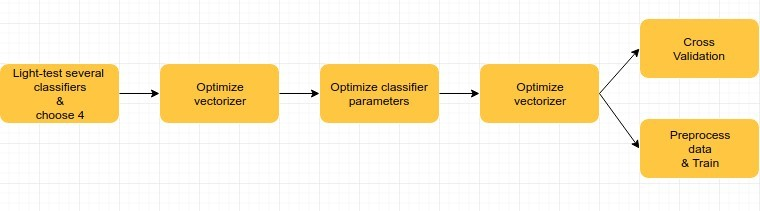
\includegraphics[width=13cm]{scikitWorkflow.jpg}
    \caption{Implementation workflow of sentiment analysis using Scikit module}%
    \label{fig:scikitWorkflow}%
\end{figure}

After manually testing and playing around with all sci-kit classifiers which are mostly used for analysis of textual data, I've decided to continue working with four of them - \textbf{Logistic Regression, Linear support vector machine and 2 Naive Bayes classifiers for multinomial models.} I had high expectations especially from Bernoulli NB as it should perform better on shorter texts. I've measured their accuracy on Sentiment140 as well as movie reviews dataset. Just out of pure curiosity I've tried to train the classifiers on movie reviews and test them on tweets contained in Sentiment140. Obviously, such approach is not correct but I wanted to see how much worse will the classifiers perform. All metrics can be seen in table \ref{table:scikitOnSentiment140}.

\paragraph{Vectorizer and its optimizations}
Goal of this step is to find best performing vectorizer for feature extraction.	Vectorization is a step when "words are turned into numbers". While words can be transformed into numbers, an entire document can be translated into a vector. Not only can a vector have more than one dimension, but with text data vectors are usually high-dimensional. This is because each dimension of your feature data will correspond to a word, and the language in the documents you are examining will have thousands of words.

The most common and simplest vectorizer approach is \textbf{bag of words}.	In this approach, union of all the words from all documents in the corpus is the dimension of the vector which is created. That means that 800 words with no duplicates would translate to an documents with 1000 words would result in 1000-dimensional vector where every unique word has its own index in that vector. Every document is processed with so called "one-hot" encoding where basically every word in the corpus is looked up in the document and zero/one is assigned accordingly. It results to every document being represented by zeros and ones. This approach has been used in my classifier built with NLT python module described in previous section. Bag of words approach is naïve in the sense that it does not distinguish the context of how a sentence or paragraph is structured. It pays attention to frequency of words but completely ignores things like position of the word in the sentence. The solution for this are N-grams. Using N-grams, vector is encoded for various combinations of words rather than just single words. This helps to preserve semantic meaning better but also causes the vector dimensionality increase. Bag of Words also can’t tell you whether or not words are unique, as the fact that a word is showing up repeatedly within a certain type of document can hint at its importance. Solution for this problem is to employ \textbf{Term Frequency-Inverse Document Frequency (TFIDF) Matrix} as a vectorization approach. That's also the vectorizer I have used for my classifier. TFIDF allows to place more emphasis on infrequent words by assigning a weight to each word instead of a binary value. The weight is determined through a combination of the word’s frequency in a document, and how rare the word is in the entire corpus.

Once I've decided which vectorizer class to use, there is also a question which parameters should I use it with. Sci-kit module offers “GridSearchCV” class which is a way how to conveniently find the best combination of all specified vectorizer parameter values. Altogether were tested and evaluated 92 vectorizers. Testing method and values examined can be seen in the following listing \ref{lst:vectorizerGridsearchcv}. 

\begin{lstlisting}[caption={Tuning of vectorizer using “GridSearchCV” class },label={lst:vectorizerGridsearchcv},language=Python]
    def tuneVectorizerParameters(corpus,labels):
    	pipeline = Pipeline([
        	('tfidf', TfidfVectorizer(stop_words='english')),
        	('clf', LinearSVC()),
    	])
    	parameters = {
        'tfidf__max_df': (0.75, 0.9),
        'tfidf__ngram_range': [(1, 1), (1, 2), (1, 3)],
        'tfidf__sublinear_tf': (True, False),
        'tfidf__stop_words':['english']
    }

    grid_search_tune = GridSearchCV(pipeline, parameters, cv=2, n_jobs=2, verbose=3)
    print("Searching best parameters combination:")
    grid_search_tune.fit(corpus, labels)

    print("Best parameters set:")
    print grid_search_tune.best_estimator_.steps
\end{lstlisting}

\paragraph{Classifier optimizations}
All classification algorithms have several parameters which can adjust and possibly improve their performance. Choosing the correct parameters for machine learning algorithms or so called “tuning” process is a field in itself and separate thesis could be written just about this. I have again used GridSearchCV class for this. For all algorithms, I have specified various values for several parameters, but even the performance for returned best parameter combination performed worse than the default parameters which are used in default constructor. Optimization of classifiers using “GridSearchCV” is briefly shown in the listing \ref{lst:classifierGridsearchcv}.

\begin{lstlisting}[caption={Tuning of classifiers using “GridSearchCV” class },label={lst:classifierGridsearchcv},language=Python]
    	scores = ['accuracy']
        # Set the parameters to combine
        SVC_parameters = [{'C': [1,10,100,1000],
                             'loss': ['hinge','squared_hinge'],
                             'multi_class': ['ovr','crammer_singer'],
                             'fit_intercept': [True,False]
                             }]
        MultiNB_parameters = [{'alpha': [1.0, 2.0, 5.0, 10.0],
                             'fit_prior': [True, False]
                             }]
        BernoulliNB_parameters = [{'alpha': [1.0, 2.0, 5.0, 10.0],
                                   'binarize': [0.0, 2.0, 5.0, 10.0],
                                 'fit_prior': [True, False]
                                 }]

        for score in scores:
            print("Tuning hyper-parameters for %s" % score)

            clf = GridSearchCV(LinearSVC(), SVC_parameters, cv=5,scoring='%s' % score)
            clf.fit(train_corpus_tf_idf, y_train)

            print("Best parameters set found:")
            print(clf.best_params_)
            print("Performance for all combinations:")
            means = clf.cv_results_['mean_test_score']
            stds = clf.cv_results_['std_test_score']
            for mean, std, params in zip(means, stds, clf.cv_results_['params']):
                print("%0.3f (+/-%0.03f) for %r"
                      % (mean, std * 2, params))

            print("Detailed classification report of model trained and evaluated on full dev/eval sets:")
            y_true, y_pred = y_test, clf.predict(test_corpus_tf_idf)
            print(classification_report(y_true, y_pred))
\end{lstlisting}    


\begin{table}[H]
\centering
\begin{tabular}{| p{3cm}|p{3cm}|p{5cm}|p{3cm}|}
 \hline
\textbf{ Training data }& \textbf{Test data} & \textbf{ Classifier }& \textbf{Accuracy}\\
 \hline
  \multirow{4}{*}{Sentiment140}   & \multirow{4}{*}{Sentiment140} & Linear SVM   & 0.785\\ 
    &  &  Multinomial Naive Bayes & 0.761\\ 
    &  &  Bernoulli Naive Bayes & 0.773\\  
    &  & Logistic Regression & 0.797\\ \hline 
  \multirow{4}{*}{Movie reviews}   & \multirow{4}{*}{Movie reviews} & Linear SVM   & 0.849\\ 
    &  &  Multinomial Naive Bayes & 0.807\\ 
    &  &  Bernoulli Naive Bayes & 0.792\\  
    &  & Logistic Regression & 0.823\\ \hline 
  \multirow{4}{*}{Movie reviews}   & \multirow{4}{*}{Sentiment140} & Linear SVM   & 0.560\\ 
    &  &  Multinomial Naive Bayes & 0.562\\ 
    &  &  Bernoulli Naive Bayes & 0.5\\  
    &  & Logistic Regression & 0.515\\ \hline 
\end{tabular}
\caption{Scikit classifiers accuracy on Sentiment140 dataset}
\label{table:scikitOnSentiment140}
\end{table}

As we can see, performance of these classifiers is much better than the previous one using Textblob. Despite 78\% accuracy might still sound pretty low, it's important to realize that Tweets are very short text pieces which often don't offer much sentiment input to work with. Therefore is 78\% quite promising performance for future work. For example, other paid services like MonkeyLearn \footnote{https://monkeylearn.com/} offer 81\% accuracy on Tweets sentiment classification.

Another thing I tried to increase the accuracy of the classifiers was preprocessing. First I have kept only words which contained only letters and then I have decided to get rid also of urls, punctuation, usernames and hastags. Accuracy metrics can be seen in table \ref{table:preprocesingAccuracy}. Training and testing data were from Sentiment140. Performance boost was smaller that expected but still, any improvement is better than none.

\begin{table}[H]
\centering
\begin{tabular}{|p{5cm}|p{5cm}|p{3cm}|}
 \hline
\textbf{Preprocessing type} & \textbf{ Classifier }& \textbf{Accuracy}\\
 \hline
 \multirow{4}{*}{\parbox{5cm}{\centering Just words with letters}} & Linear SVM   & 0.785\\ 
   &  Multinomial Naive Bayes & 0.76\\ 
   &  Bernoulli Naive Bayes & 0.772\\  
   & Logistic Regression & 0.796\\ \hline 
  \multirow{4}{*}{\parbox{5cm}{\centering Stripped URLs, punctuation, usernames, alphanumetric characters, hashtags}} & Linear SVM   & 0.786\\ 
   &  Multinomial Naive Bayes & 0.766\\ 
   &  Bernoulli Naive Bayes & 0.774\\  
   & Logistic Regression & 0.795\\ \hline 
\end{tabular}
\caption{Scikit classifiers accuracy on Sentiment140 dataset}
\label{table:preprocesingAccuracy}
\end{table}


\paragraph{Neutral Tweets}: At this point, after all the tuning, optimizing and cross-validation, I could finally run my analyzer on the testdata also provided by Sentiment140. Compared to the training data which contain just positive and negative tweets, test file contains also neutral ones. Obviously, this is a problem, since my classifiers are not familiar with the concept of neutral tweets. In current state, accuracy on a test set with neutral tweets is just 58.4\% whereas on the same test set with excluded neutral tweets, accuracy was more than 81\% - which is expected because it's basically the same set just with different tweets which has also been used	 during cross-validation. 

In general, third neutral class in sentiment analysis is still causing big problems. E.g Go, Huang and Bhayani \cite{go2009twitter2} considered any tweet without an emoticon to be part of the neutral class, which they themselves admitted to be a flawed approach. Kouloumpi at al. \cite{kouloumpis2011twitter} trained their classifier just on hashtags and emoticons and also had to build their own neutral training dataset.  Agarwal at al \cite{agarwal2011sentiment} annotated their own training dataset to contain neutral tweets and achieved very nice accuracy of 60\% which is much higher than the base line of 33\%. Although it is a nice result, they had training data which contained neutral data. Saif et al. \cite{saif2012semantic} as well as Go, Huang and Bhayani \cite{go2009twitter} in their second article that year just stated that identifying neutral tweets is part of their future work plan.  Afer realizing that doing a tree way analysis rather than just binary or qualitative (output is a score value) analysis is worth a separate thesis I have decided to train my classifier for only weighted qualitative output in interval from 0 to 1, where 1 is the most positive. Just out of curiosity, I've     defined confidence thresholds for positive and negative tweets. Everything which would be between these 2 threshold levels could be considered a neutral tweet. I manually tried several values and accuracy scores from these measuments are recorded in table \ref{table:negativeAccuracy}. I've achieved accuracy just 7\% above the baseline at most, so the lack of optimization for neutral tweets classification is obvious.


\begin{table}[H]
\centering
\begin{tabular}{|p{4cm}|p{4cm}|p{3cm}|}
 \hline
\textbf{ Negative threshold }& \textbf{Positive threshold} & \textbf{Accuracy}\\
 \hline
 0.1 & 0.9 & 0.357\\ \hline
 0.2 & 0.8 & 0.385\\ \hline
 0.3 & 0.7 & 0.393\\ \hline 
 0.4 & 0.6 & 0.401\\ \hline 
\end{tabular}
\caption{Textblob accuracy with various handling of neutral tweets}
\label{table:negativeAccuracy}
\end{table}

\paragraph{Abstracting several classifiers under one custom classifier}:
I later came up with an idea of abstracting all classification algorithms all under one custom classifier. My custom classifier is able to be trained in 3 modes ways - as a binary classifier, multiclass classifier or a classifier outputting a float confidence score of text being positive.
This approach has of course both, advantages and disadvantages as well. Advantage for sure is that possibility of False positives or False Negatives is much lower as this requires 3 incorrect classifications to instead of 1. Trade-off for this is that the confidence score of being positive is in general lower because the possibility of at least one of 3 algorithms being wrong is (obviously) higher than if there is only one single classifier.

All performance matrices of the final classifier for various datasets are displayed in figure \ref{fig:finalClassifierPerformanceBarChart}


\begin{figure}[H]%
    \centering
	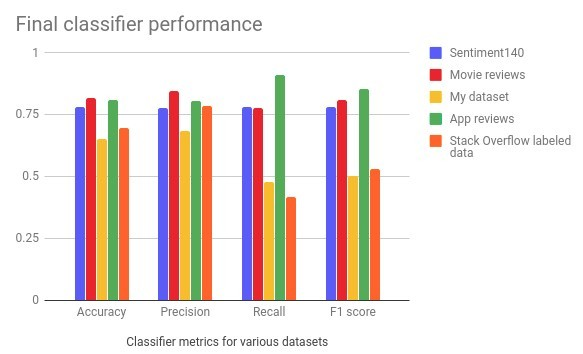
\includegraphics[width=14cm]{finalClassifierPerformanceBarChart.jpg}
    \caption{Final classifier performance for several datasets}%
    \label{fig:finalClassifierPerformanceBarChart}%
\end{figure}

It's clear that the best results are achieved with movie or app reviews because these texts offer more features to draw the sentiment from because they are longer texts. We can also see that training datasets built from shorter texts (My twitter dataset or SO labeled dataset created and used in Bin Li's paper ) have worse performance, especially recall. With my own dataset, its size might be causing this as it contains only 84 labeled entries. I concluded that using Sentiment140 as a definitive training dataset is a good choice as its performance is just sligthly worse compared to reviews but it's still authentic Twitter data which I'm going to analyze the most.